\documentclass{standalone}
\pagestyle{empty}
\usepackage{tkz-berge}
\usepackage{graphicx}
%\usepackage{pgf}

\begin{document}

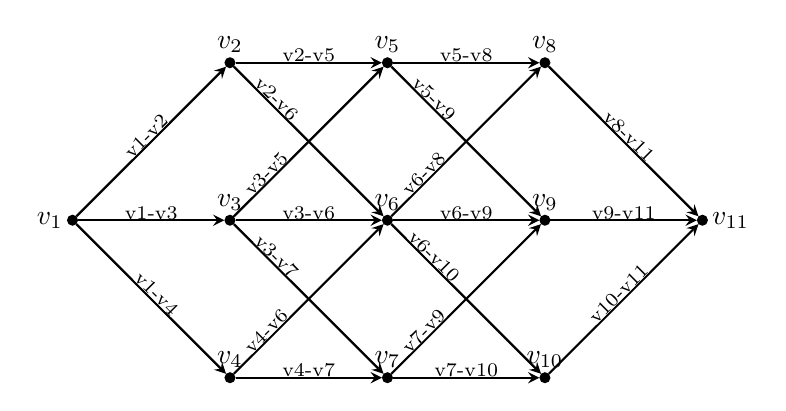
\begin{tikzpicture}[>=stealth]
  \GraphInit[vstyle=Classic]
  \SetVertexNoLabel
\SetUpVertex[Lpos=-180]
\tikzset{VertexStyle/.style = {shape=circle, fill=black,
                               minimum size=4pt,inner sep=0pt}
  }
\begin{scope}[rotate=90]
\grEmptyPath[Math, prefix=a, RA=2, RS=8, form=2]{1}
\grEmptyPath[Math, prefix=b, RA=2, RS=6, form=2]{3}
\grEmptyPath[Math, prefix=c, RA=2, RS=4, form=2]{3}
\grEmptyPath[Math, prefix=d, RA=2, RS=2, form=2]{3}
\grEmptyPath[Math, prefix=e, RA=2, RS=0, form=2]{1}
\end{scope}

\tikzset{EdgeStyle/.style={->, ,font=\scriptsize,above,sloped,midway,inner sep=0pt}}

\Edge[label=v1-v4](a0)(b0)
\Edge[label=v1-v3](a0)(b1)
\Edge[label=v1-v2](a0)(b2)
%-----------------------------
\Edge[label=v4-v7](b0)(c0)
\Edge[label=v3-v6](b1)(c1)
\Edge[label=v2-v5](b2)(c2)
%-----------------------------
\Edge[label=v7-v10](c0)(d0)
\Edge[label=v6-v9](c1)(d1)
\Edge[label=v5-v8](c2)(d2)
%-----------------------------
\Edge[label=v10-v11](d0)(e0)
\Edge[label=v9-v11](d1)(e0)
\Edge[label=v8-v11](d2)(e0)

\tikzset{EdgeStyle/.style={->, ,font=\scriptsize,above,sloped,near start,inner sep=0pt}}

\Edge[label=v4-v6](b0)(c1)

\Edge[label=v3-v7](b1)(c0)
\Edge[label=v3-v5](b1)(c2)

\Edge[label=v2-v6](b2)(c1)
\Edge[label=v7-v9](c0)(d1)

\Edge[label=v6-v10](c1)(d0)
\Edge[label=v6-v8](c1)(d2)

\Edge[label=v5-v9](c2)(d1)


\tikzset{AssignStyle/.append style=left}
\AssignVertexLabel{a}{$v_1$}
\tikzset{AssignStyle/.append style=above}
\AssignVertexLabel{b}{$v_4$,$v_3$,$v_2$}
%\tikzset{AssignStyle/.append style=above}
\AssignVertexLabel{c}{$v_7$,$v_6$,$v_5$}
\AssignVertexLabel{d}{$v_{10}$,$v_9$,$v_8$}
\tikzset{AssignStyle/.append style=right}
\AssignVertexLabel{e}{$v_{11}$}

\end{tikzpicture}

\end{document}